% Risultati per test a grafo crescente in numero di nodi
    % tutte le versioni sia su diretti che indiretti
        % grafici confronto
        % commenti
    
% Risultati per test a grafo con densità crescente
    % grafico
    % osservazioni e possibii spiegazioni
        % con matrice tempo costante perché ...
        % con BCSR tempo crescente con densità perché ...
        % per densità elevate stessi tempi
        % linea viola bcsr senza ottimizzazioni work balance (inutile)
        


\chapter{Risultati}\label{chap:Risultati}

    In questo capitolo verranno discussi i principali risultati riscontrati durante la fase di testing. 

    Per facilitare la lettura dei grafici, si ricorda che:
    \begin{description}
        \item[{\color{blue}serial}] è la versione seriale, la prima implementata;
        \item[{\color{red}parallel}] è la prima versione parallela, i grafi sono rappresentati tramite matrice di adiacenza;
        \item[{\color{violet}parallelbcsrtc}] è la seconda versione parallela, molto simile alla precedente, viene adattata per la rappresentazione BCSR includendo le ottimizzazioni che quest'ultima consente;
        \item[{\color{YellowOrange}parallelbcsrvc}] è l'ultima versione implementata, la versione \textit{work balanced}, e applica alla versione precedente diverse ottimizzazioni per sfruttare al massimo le risorse computazionali.
    \end{description}

    Nella prima parte metteremo a confronto le varie implementazioni su input in cui il numero di nodi è variabile e la densità è costante. 
    Viceversa, nella seconda parte analizzeremo come la variazione di densità influisce sui tempi di esecuzione.

    \section{Risultati per quantità nodi variabile}

        Di seguito sono riportati due grafici che mettono a confronto le diverse implementazioni sia nel caso di grafi diretti (Figura \ref{fig:exec-time-dir}) che in quello di grafi indiretti (Figura \ref{fig:exec-time-undir}). I grafici rappresentano esclusivamente i tempi di esecuzione dell'algoritmo, sono esclusi quindi i tempi di inizializzazione e salvataggio dei risultati.

        I valori di tutti gli assi sono espressi in scala logaritmica. Altrimenti, vista la grande differenza tra i valori, alcune linee risulterebbero appiattite e sovrapposte, rendendo difficile l'analisi dei risultati.

        Sulle ordinate sono riportati i tempi espressi in millisecondi mentre sulle ascisse il numero di nodi.

        Prima di passare alle osservazioni sui grafici, facciamo notare che non tutte le versioni sono state testate su tutte le istanze a disposizione per i seguenti motivi:
        \begin{itemize}
            \item la versione seriale è risultata essere talmente inefficiente (in termini di tempo) da consentirne l'esecuzione solamente con piccole istanze;
            \item la prima versione parallela, usando la matrice di adiacenza come metodo di rappresentazione dei dati, è risultata limitata nell'utilizzo della memoria al punto da renderne impossibile l'esecuzione su istanze con più di 30mila nodi.
        \end{itemize}

        Dunque, osservando i grafici si nota quanto segue:
        \begin{itemize}
            \item la versione seriale risulta essere competitiva solamente quando si hanno qualche decina di nodi. Dopodiché, qualsiasi versione parallela diventa preferibile;
            \item le versioni parallele, invece, tra di loro hanno tempi comparabili per grafi di piccole dimensioni, mentre per istanze di medie/grandi dimensioni si iniziano a notare delle differenze;
            \item in generale l'implementazione migliore sembrerebbe l'ultima proposta (approccio \textit{work balanced});
            \item la versione parallela con BCSR (linea viola), all'aumentare delle dimensioni del grafo, sembrerebbe avvicinarsi ai tempi della versione parallela con matrice di adiacenza (linea rossa). Purtroppo non è possibile valutare con esattezza il loro comportamento, essendo la prima versione parallela fortemente limitata dal consumo di memoria.            
        \end{itemize}
        
        \begin{figure}
            \centering
            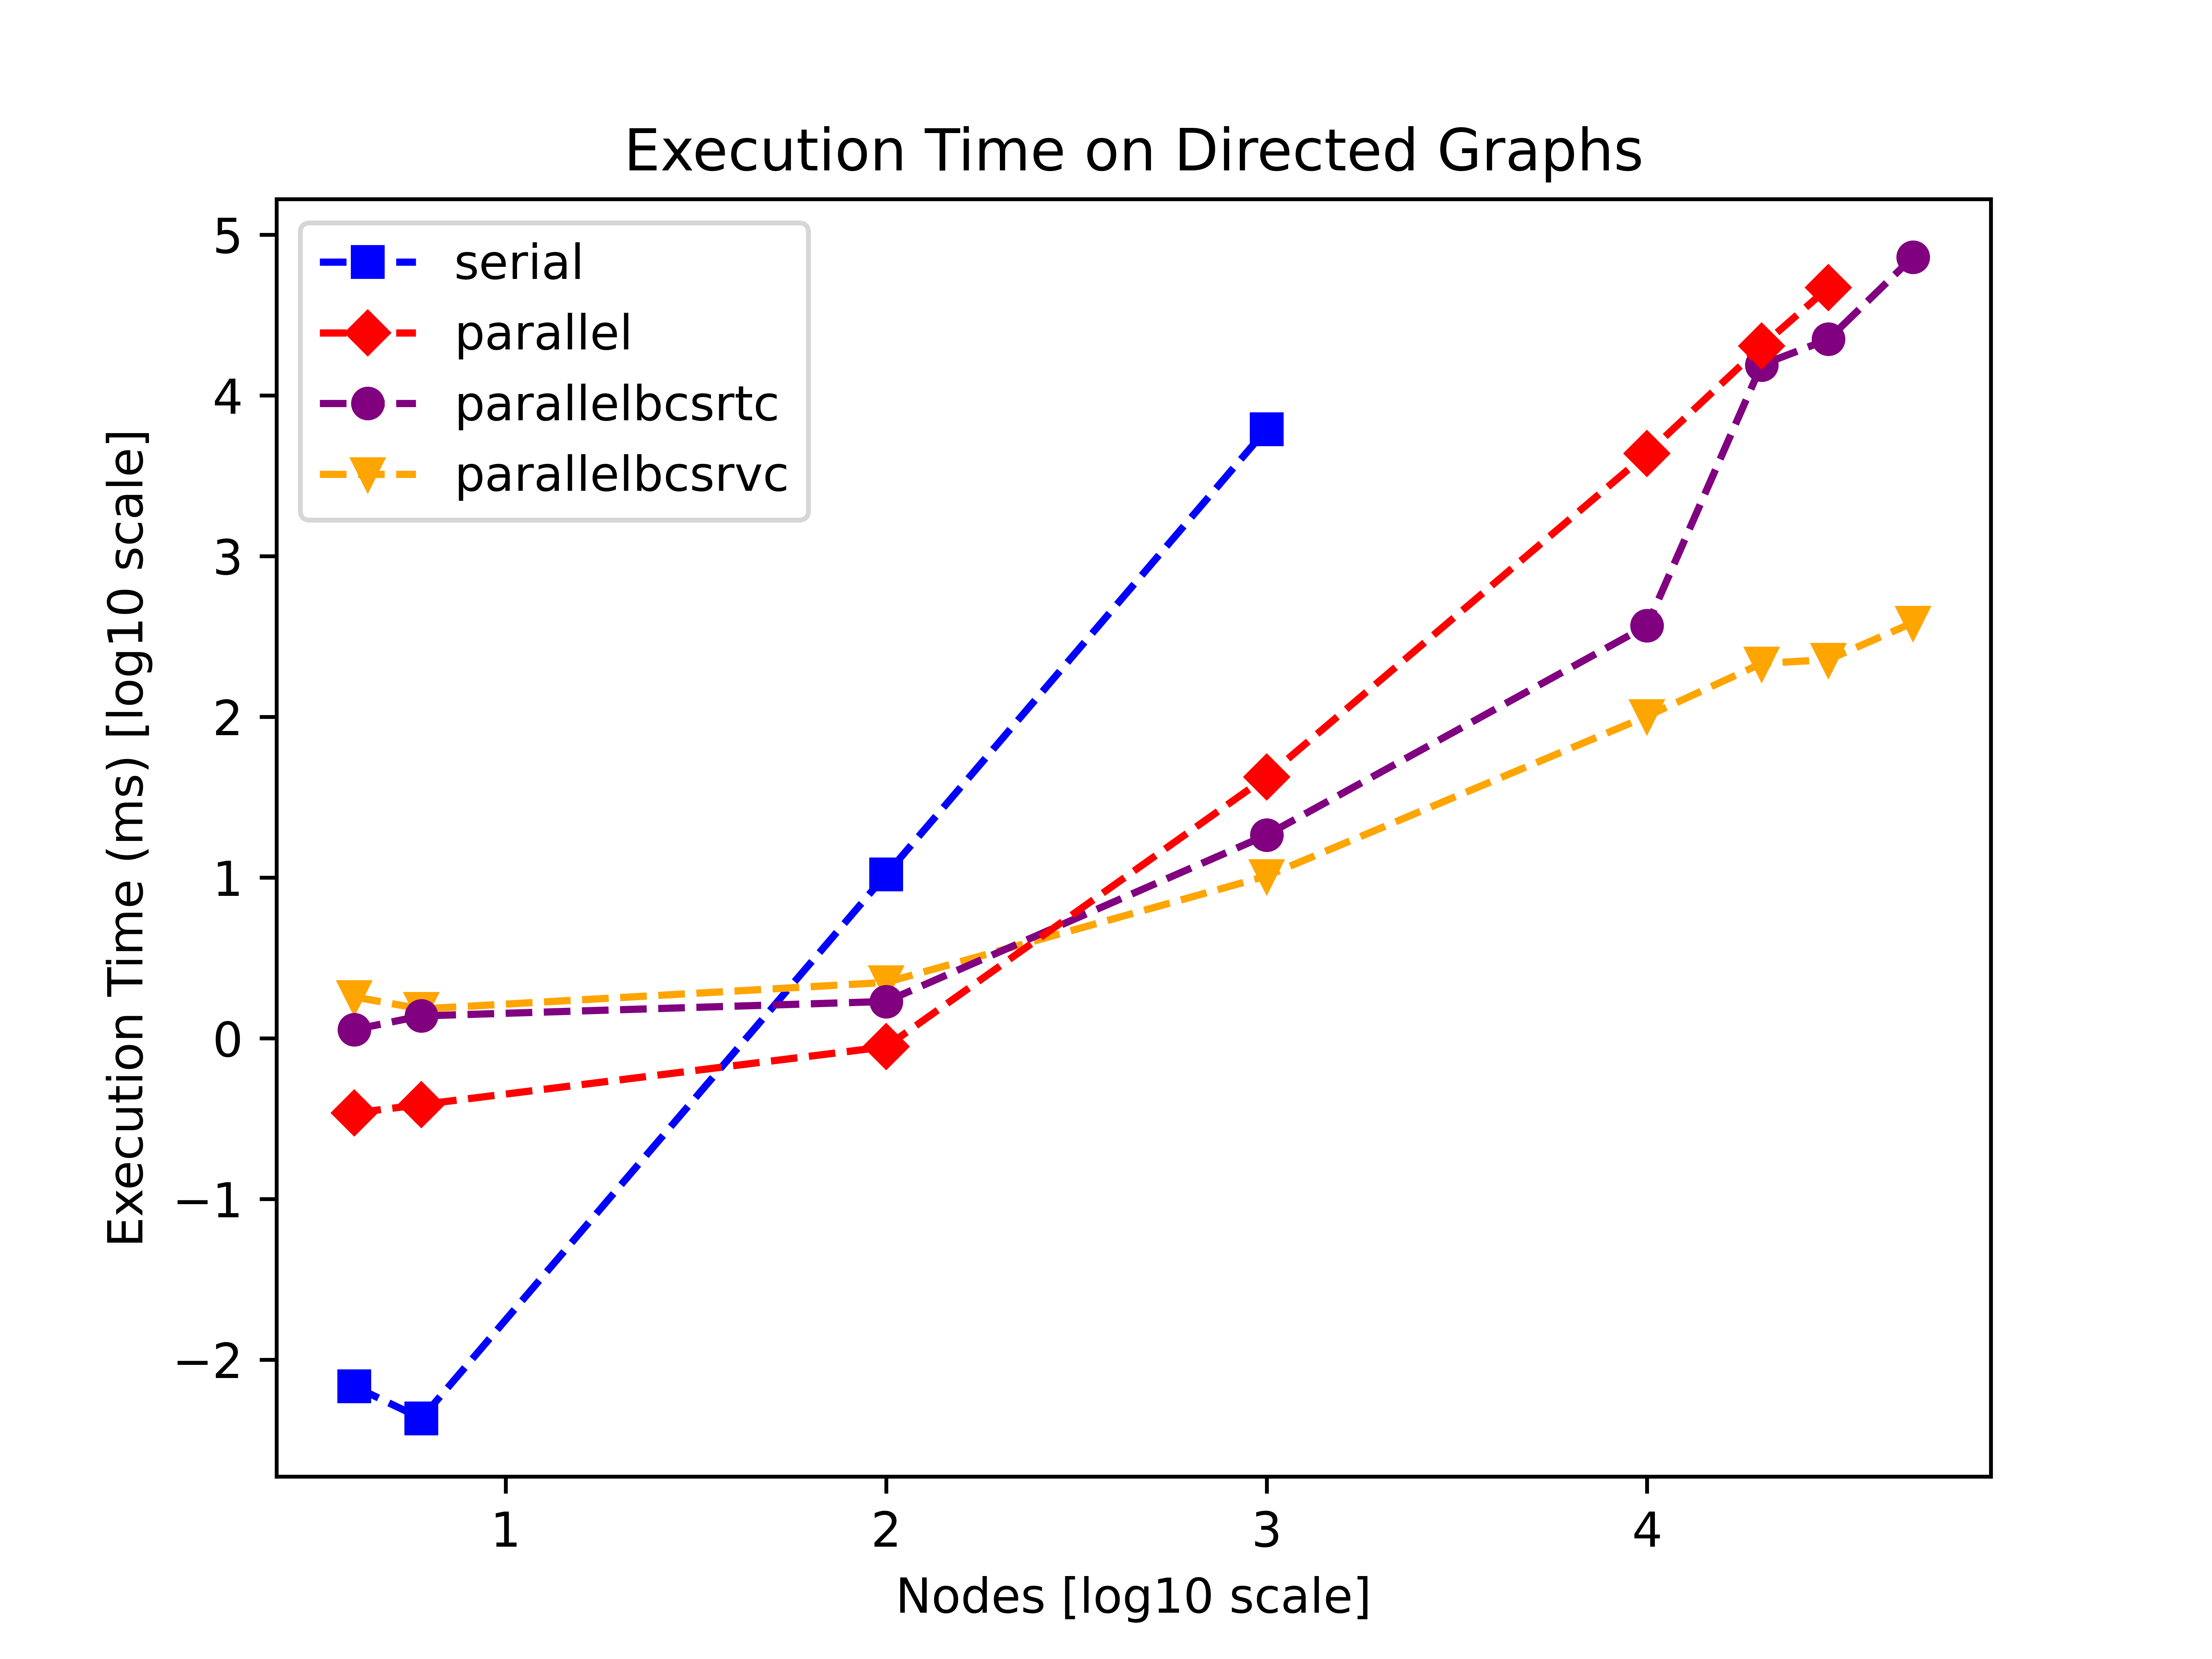
\includegraphics[width=0.7\linewidth]{images/execution_time_directed.png}
            \caption{Tempi di esecuzione con grafi diretti}
            \label{fig:exec-time-dir}
        \end{figure}
    
        \begin{figure}
            \centering
            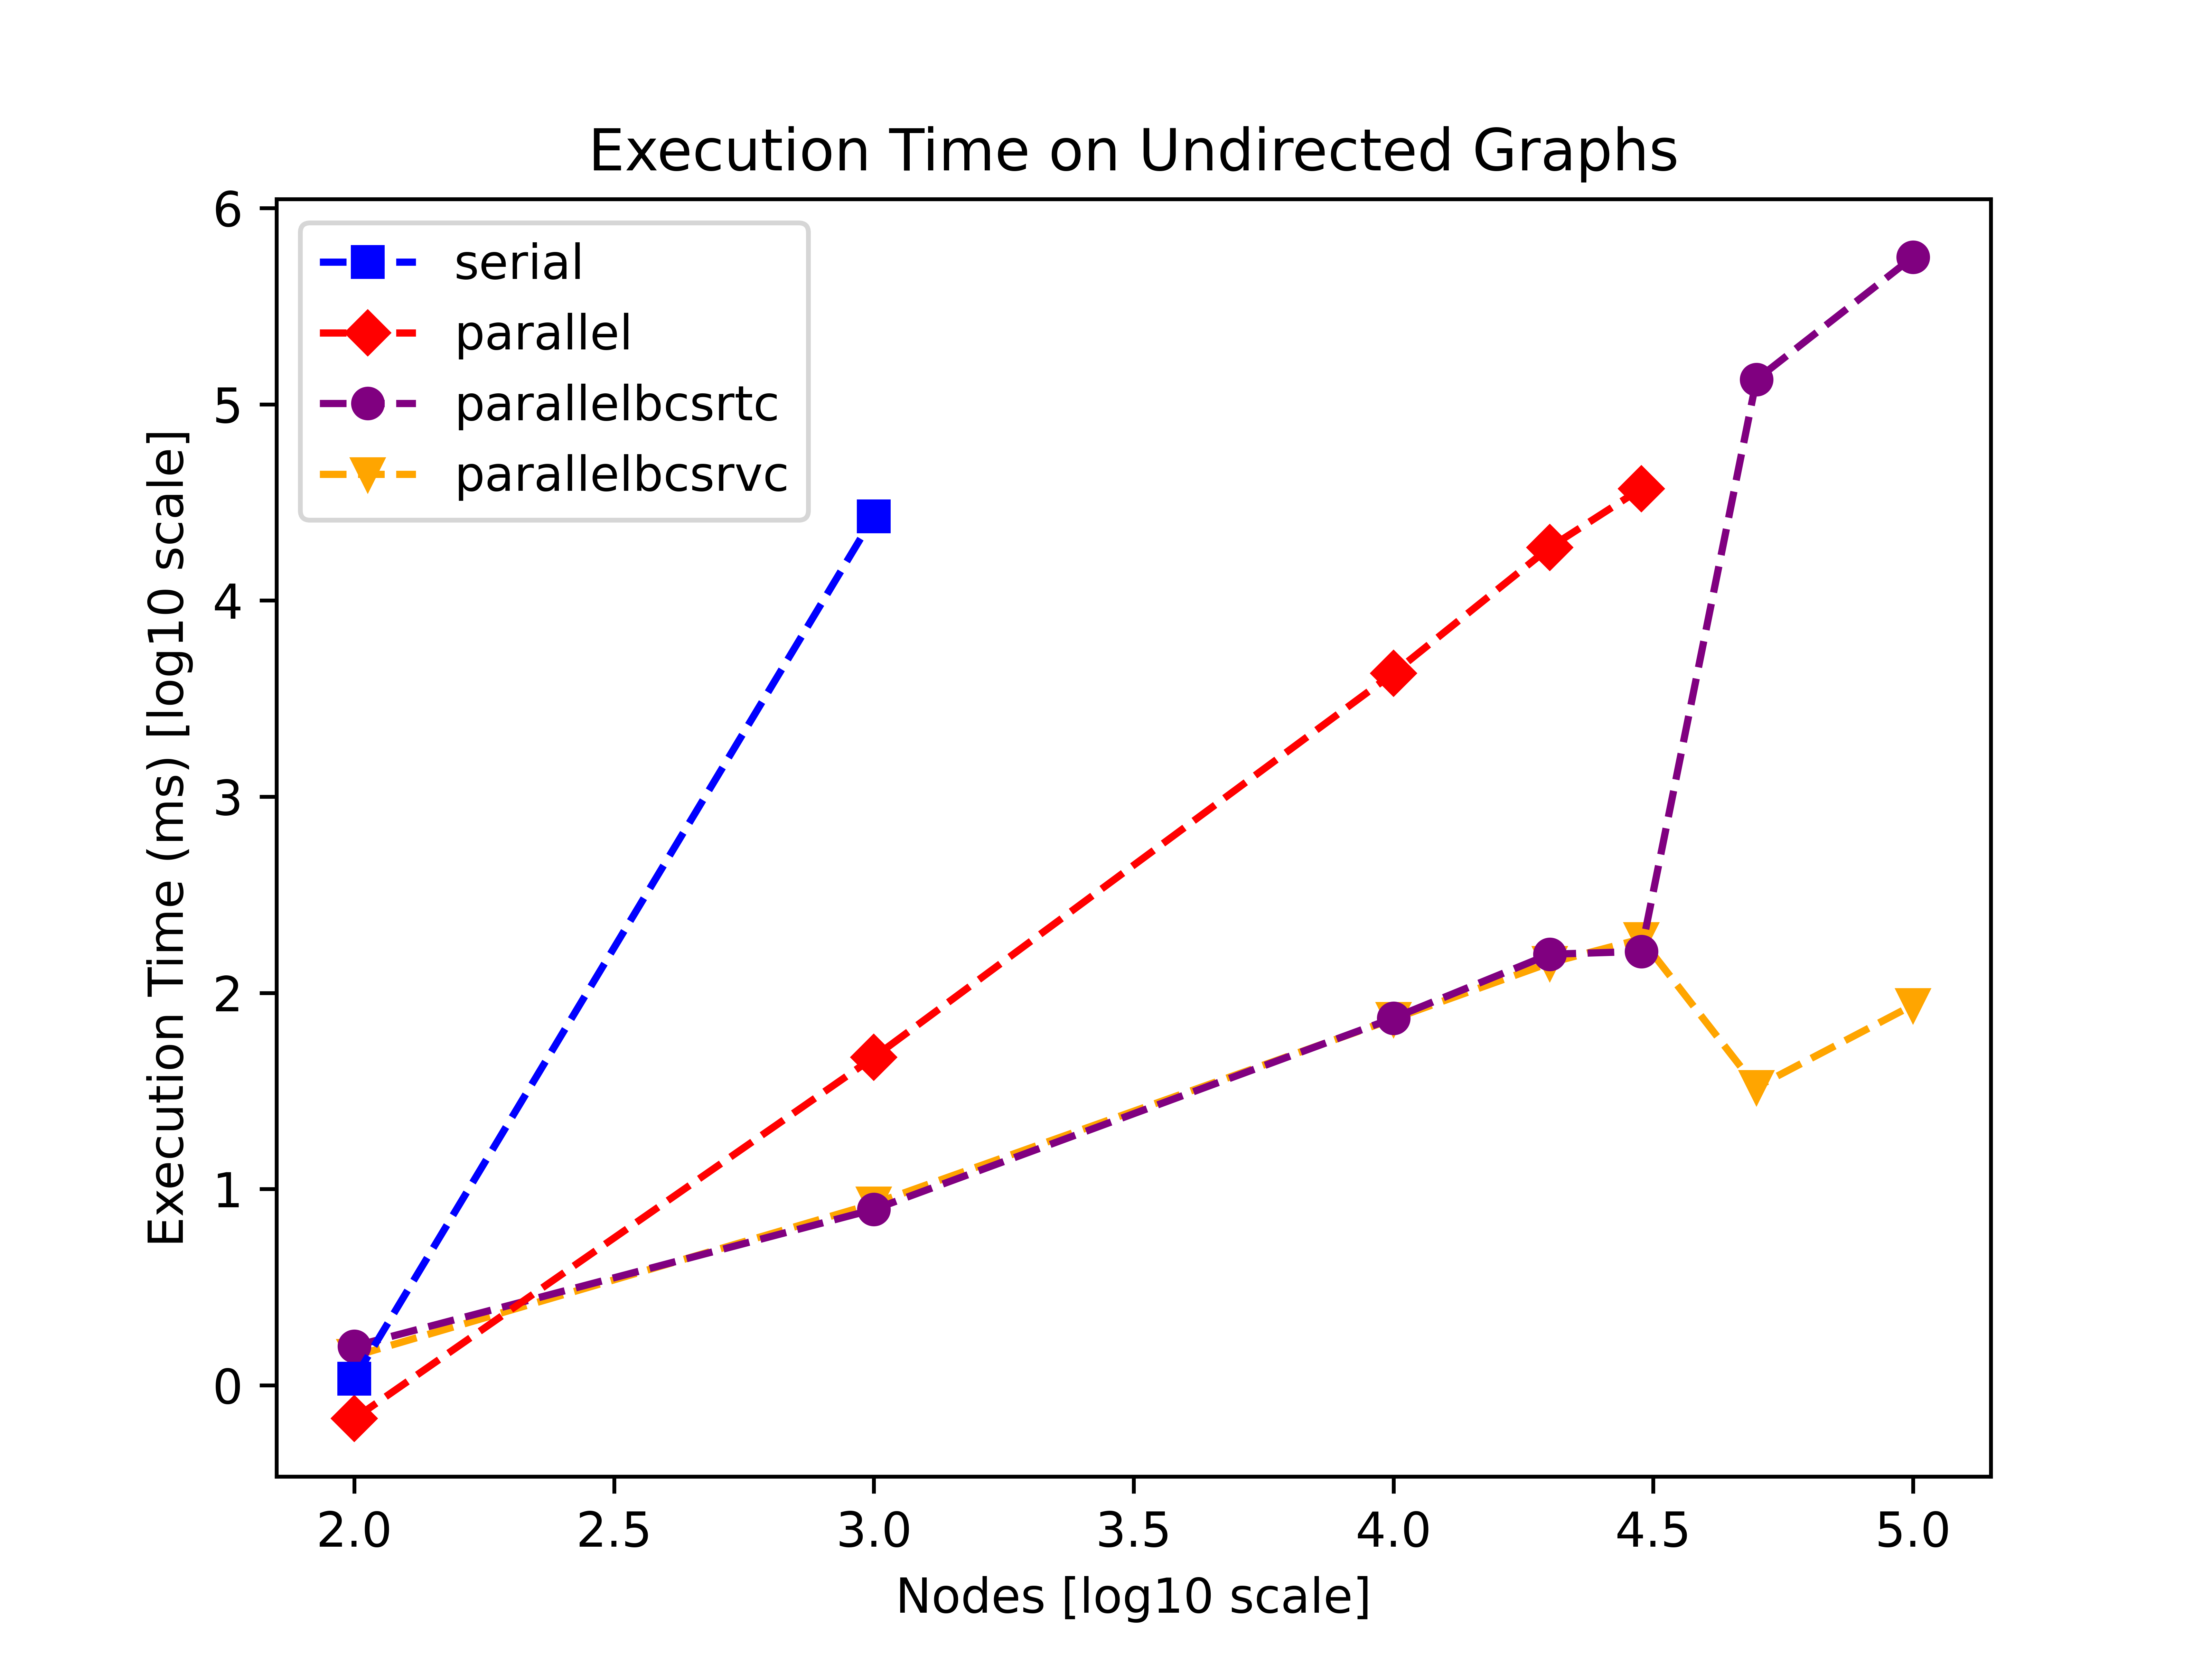
\includegraphics[width=0.7\linewidth]{images/execution_time_undirected.png}
            \caption{Tempi di esecuzione con grafi non diretti}
            \label{fig:exec-time-undir}
        \end{figure}
    
    
    \section{Risultati per densità variabile}

        In questa sezione analizziamo come la densità del grafo influisce sui tempi di esecuzione dell'algoritmo. Il grafico in Figura \ref{fig:exec-time-density} mostra i tempi di esecuzione delle diverse versioni dell'algoritmo su grafi diretti con densità variabile.

        In questo caso, sull'asse X sono riportati i valori di densità, mentre sull'asse Y i tempi di esecuzione in millisecondi. Ricordiamo che i grafi usati in input avevano un numero di nodi fisso pari a 1000 e una densità variabile tra 0.1 e 1 (grafo completo).

        \begin{figure}
            \centering
            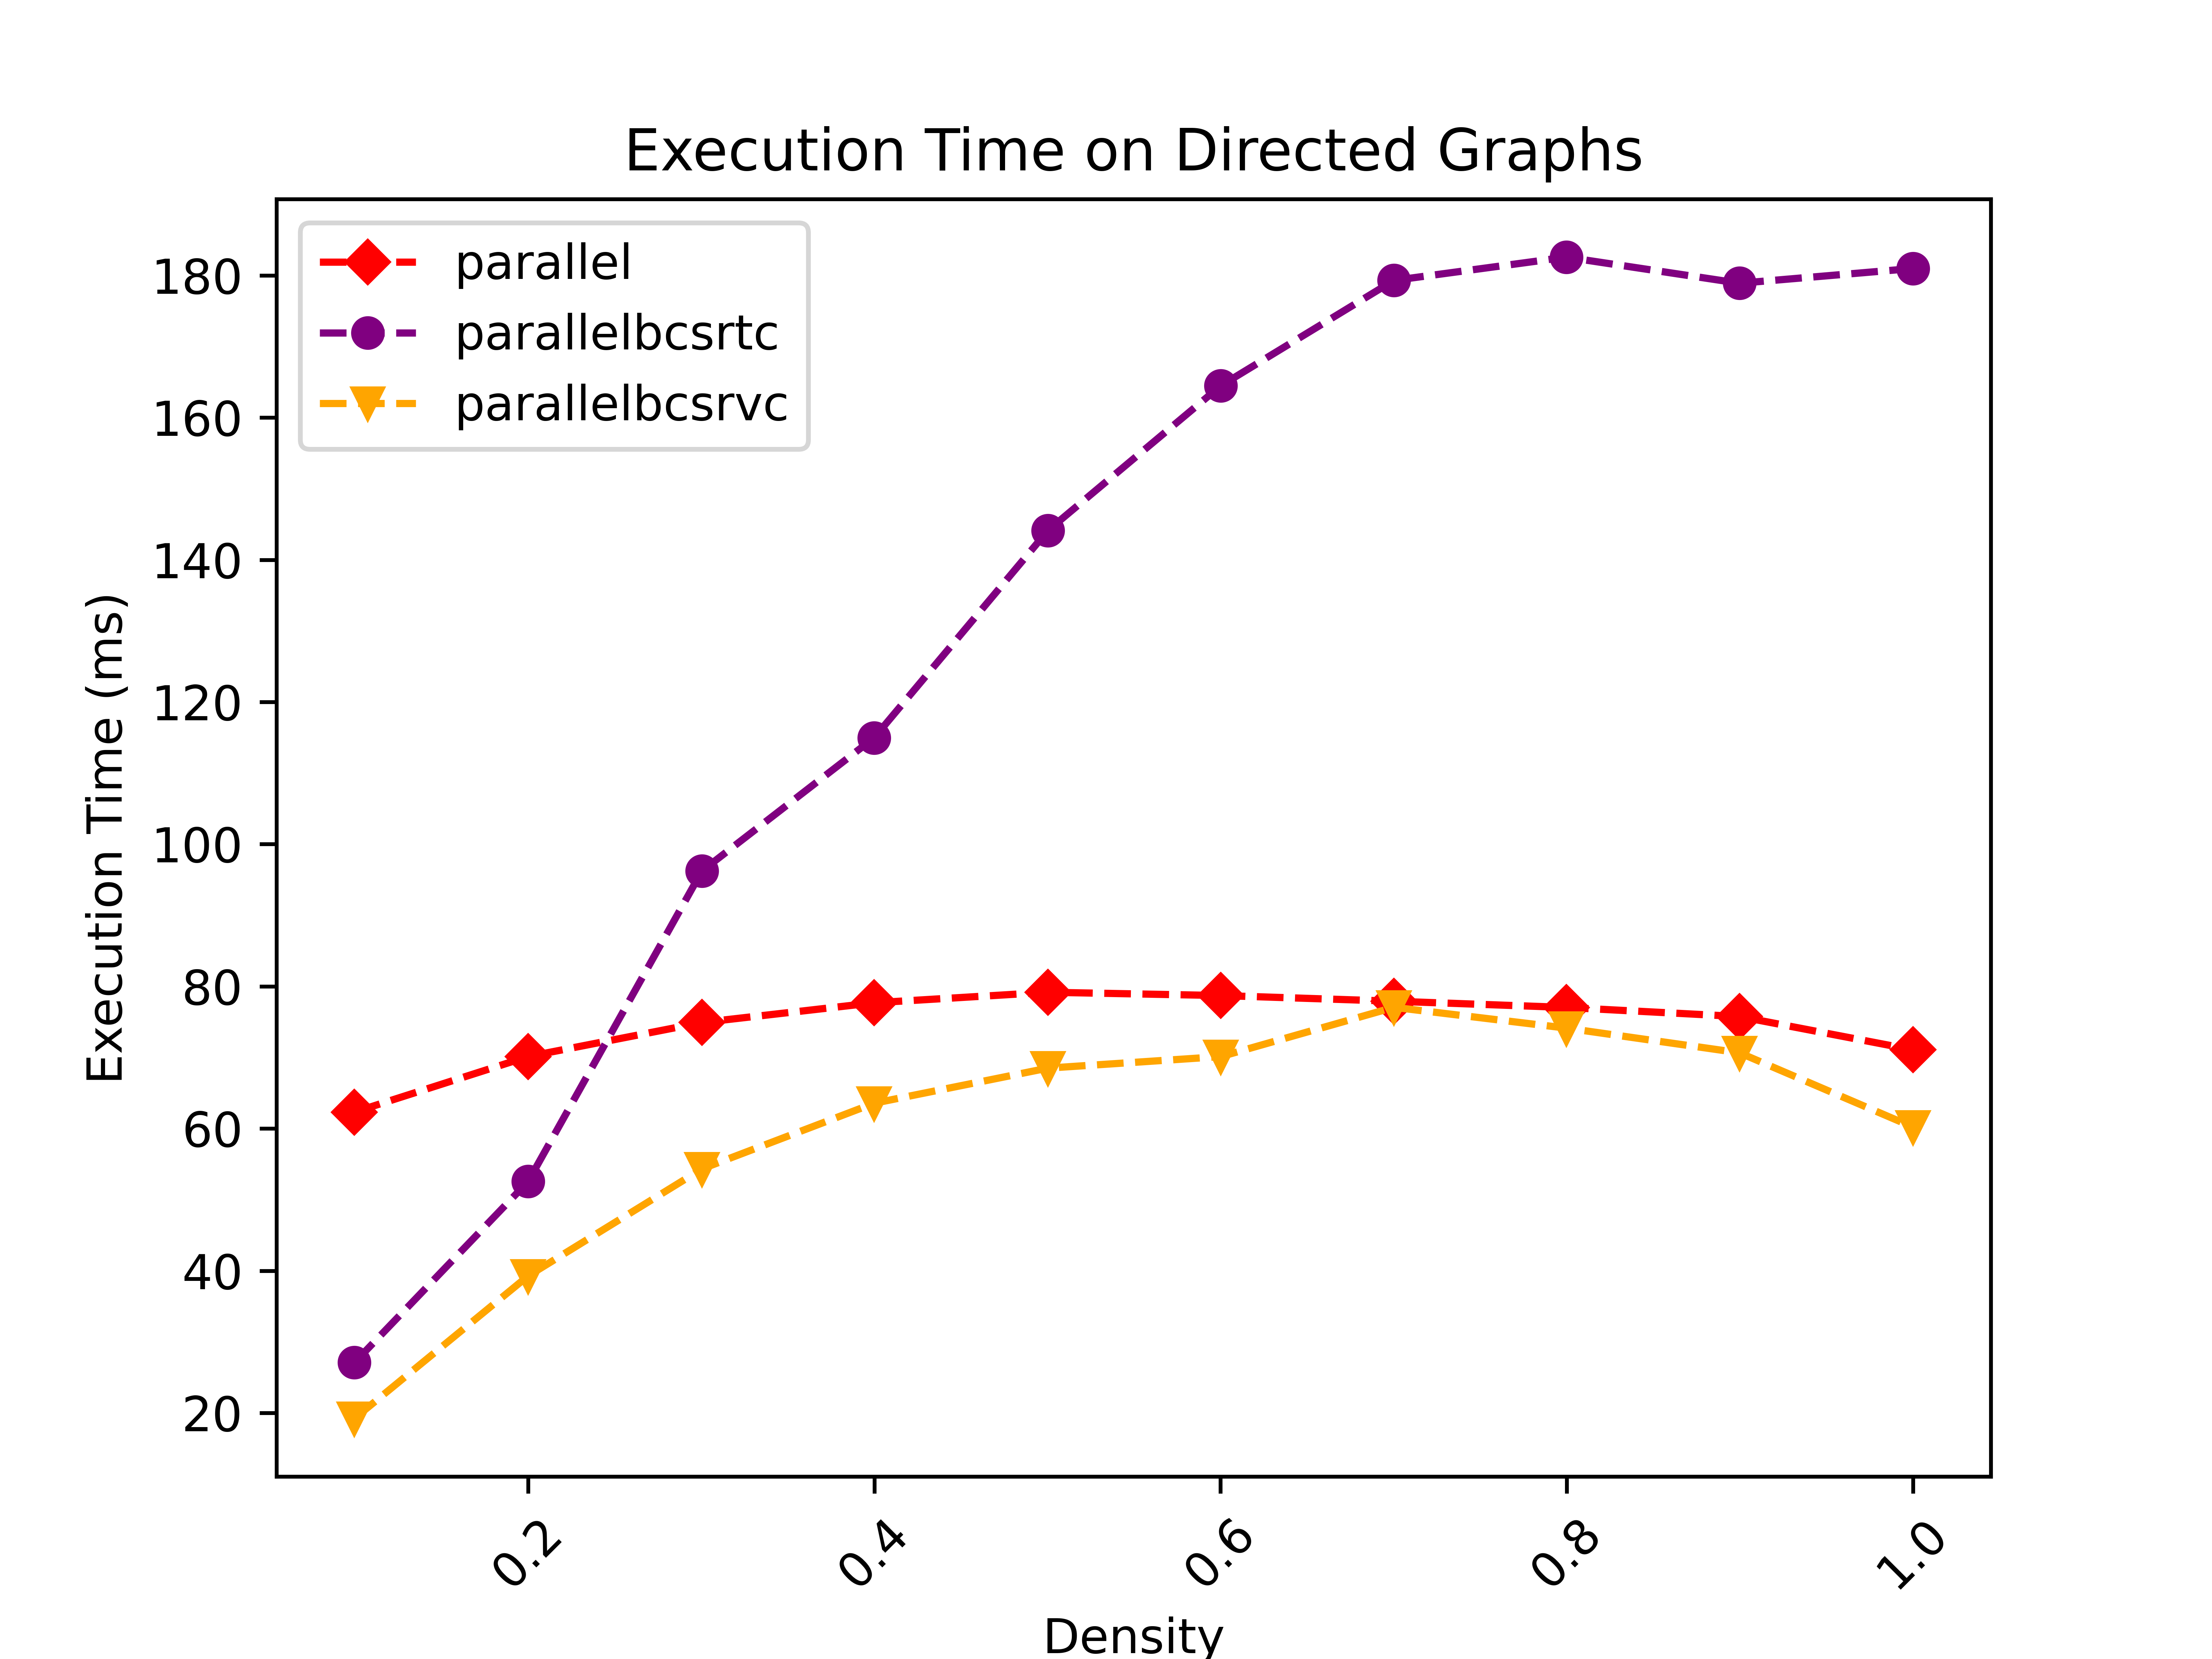
\includegraphics[width=0.7\linewidth]{images/execution_time_density.png}
            \caption{Tempi di esecuzione con grafi diretti a densità variabile}
            \label{fig:exec-time-density}
        \end{figure}

        Dal grafico si può notare che:
        \begin{itemize}
            \item la versione seriale non è presente poiché si è dimostrata essere inefficiente anche con grafi relativamente di piccole dimensioni e densità ridotta;
            \item la versione parallela con matrice di adiacenza (linea rossa) ha tempi di esecuzione pressoché costanti, indipendentemente dalla densità del grafo. Questo è dovuto al fatto che l'algoritmo che usa la matrice di adiacenza ha un costo computazionale che dipende dal numero di nodi e non dalla densità del grafo (la matrice ha sempre dimensione $|V| \times |V|$ indipendentemente dalla densità);
            \item la versione parallela con BCSR (linea viola) ha tempi di esecuzione crescenti all'aumentare della densità del grafo. Questo è dovuto al fatto che la rappresentazione BCSR è vantaggiosa per grafi sparsi e non densi. In particolare, all'aumentare della densità, lo stesso algoritmo con rappresentazione BCSR diventa meno efficiente rispetto a quello basato su matrice di adiacenza;
            \item la versione parallela \textit{work balanced} (linea gialla) ha tempi di esecuzione crescenti ma mai superiori rispetto alla versione con matrice di adiacenza. Nello specifico, questa implementazione risulta essere vantaggiosa per grafi a bassa densità, mentre i tempi risultano essere comparabili per grafi a più alta densità. Questo è dovuto al fatto che l'implementazione \textit{work balanced} combinata con la rappresentazione BCSR è ottimizzata per sfruttare al meglio le risorse computazionali.
        \end{itemize}

    \section{Considerazioni}
        I test su grafi con densità e numero di nodi crescente offrono una valutazione dettagliata dell'algoritmo Push-Relabel parallelo, evidenziando vantaggi e limiti legati sia alla natura dei grafi sia alle strutture dati.

        Con grafi a numero di nodi crescente, le versioni parallele superano presto quella seriale, con l'implementazione work-balanced che si distingue su istanze di medie e grandi dimensioni. Tuttavia, alcuni problemi come quelli legati alla memoria (ad esempio con la matrice di adiacenza) possono influire sulle prestazioni.

        Nei grafi a densità crescente, la scelta delle strutture dati da utilizzare è cruciale. La versione con matrice di adiacenza ha tempi costanti, indipendenti dalla densità, mentre la versione BCSR diventa meno efficiente con grafi densi. L'implementazione work-balanced rimane vantaggiosa nei grafi a bassa densità, ma si allinea alla matrice di adiacenza con grafi più densi.

        In sintesi, prestazioni e scalabilità dipendono dalla scelta delle strutture dati e dalla gestione del parallelismo.